\documentclass[a4paper,12pt]{article} 

%%% Работа с русским языком
\usepackage{cmap}					% поиск в PDF
\usepackage{mathtext} 				% русские буквы в фомулах
\usepackage[T2A]{fontenc}			% кодировка
\usepackage[utf8]{inputenc}			% кодировка исходного текста
\usepackage[english,russian]{babel}	% локализация и переносы

%%% Дополнительная работа с математикой
\usepackage{amsmath,amsfonts,amssymb,amsthm,mathtools, gensymb} % AMS
\usepackage{icomma} % "Умная" запятая: $0,2$    ф--- число, $0, 2$ --- перечисление

%%Таблица
\usepackage[table,xcdraw]{xcolor}
\usepackage{caption}
\usepackage{floatrow}
\floatsetup[table]{capposition=top}
\floatsetup[wrapfigure]{capposition=bottom}
\usepackage{multirow}

%Отступы и поля 
\textwidth=18cm
\oddsidemargin=-1cm
\topmargin=-2cm
\textheight=25cm


%% Номера формул
\mathtoolsset{showonlyrefs=true} % Показывать номера только у тех формул, на которые есть \eqref{} в тексте.

%% Шрифты
\usepackage{euscript}	 % Шрифт Евклид
\usepackage{mathrsfs} % Красивый матшрифт

%% Свои команды
\DeclareMathOperator{\sgn}{\mathop{sgn}}

%% Перенос знаков в формулах (по Львовскому)
\newcommand*{\hm}[1]{#1\nobreak\discretionary{}
{\hbox{$\mathsurround=0pt #1$}}{}}

%% Стиль страницы
\usepackage{fancyhdr}

%% Для рисунков
\usepackage{graphicx}
\usepackage[export]{adjustbox}
\usepackage{float}
\usepackage{ragged2e}
\usepackage{wrapfig}

\pagestyle{fancy}
\begin{document}
\begin{titlepage}
\begin{center}
%\vspace*{1cm}
\large{\small ФЕДЕРАЛЬНОЕ ГОСУДАРСТВЕННОЕ АВТОНОМНОЕ ОБРАЗОВАТЕЛЬНОЕ\\ УЧРЕЖДЕНИЕ ВЫСШЕГО ОБРАЗОВАНИЯ \\ МОСКОВСКИЙ ФИЗИКО-ТЕХНИЧЕСКИЙ ИНСТИТУТ\\ (НАЦИОНАЛЬНЫЙ ИССЛЕДОВАТЕЛЬСКИЙ УНИВЕРСИТЕТ)\\ ФАКУЛЬТЕТ АЭРОКОСМИЧЕСКИХ ТЕХНОЛОГИЙ}
\vfill
\line(1,0){490}\\[1mm]
\huge{Лабораторная работа 4.7.3}\\
\huge\textbf{Изучение поляризованного света}\\
\line(1,0){490}\\[1mm]
\vfill
\begin{flushright}
\normalsize{Рогозин Владимир}\\
\normalsize{\textbf{Группа Б03-106}}\\
\end{flushright}
\end{center}
\end{titlepage}
\fancyhead[L] {Работа 4.7.3}

\textbf{Цель работы}:
ознакомление с методами получения и анализа поляризованного света.

\textbf{Оборудование}:
оптическая скамья с осветителем; зеленый светофильтр; два поляроида; черное зеркало; полированная эбонитовая пластинка; стопа стеклянных пластинок; слюдяные пластинки разной толщины; пластинки в $1/4$ и $1/2$ длины волны; пластинка в одну длину волны для зеленого света (пластинка чувствительного оттенка).

\section{Теоретические сведения}

\subsection{Естественный и поляризованный свет}
Как известно, световые волны поперечны: электрический вектор $\mathbf{E}$ и магнитный вектор $\mathbf{H}$ взаимно перпендикулярны и располагаются в плоскости, перпендикулярной направлению распространения волны. Во всякой данной точке пространства ориентация пары векторов $\mathbf{E}$ и $\mathbf{H}$ в плоскости, перпендикулярной лучу $\mathbf{S}$, может, вообще говоря, изменяться со временем.
В зависимости от характера такого изменения различают естественный и поляризованный свет.

Обычные источники света являются совокупностью огромного числа быстро высвечивающихся элементарных источников (атомов или молекул), испускающих свет независимо друг от друга, с разными фазами и с разными ориентациями векторов $\mathbf{E}$ и $\mathbf{H}$. Ориентация векторов $\mathbf{E}$ и $\mathbf{H}$ в результирующей волне поэтому хаотически изменяется во времени, так что в плоскости, перпендикулярной лучу $\mathbf{S}$, все направления оказываются в среднем равноправными. Такой свет называют \textit{естественным} или \textit{неполяризованным}.

При помощи специальных приспособлений (поляризаторов) естественный свет может быть превращен в линейно поляризованный. В \textit{линейно поляризованной} световой волне пара векторов $\mathbf{E}$ и $\mathbf{H}$ не изменяет с течением времени своей ориентации. Плоскость $\mathbf{E}$, $\mathbf{S}$ называется в этом случае \textit{плоскостью колебаний}.

Наиболее общим типом поляризации является эллиптическая поляризация. В \textit{эллиптически поляризованной} световой волне конец вектора $\mathbf{E}$ описывает некоторый эллипс. Линейно поляризованный свет можно рассматривать как частный случай эллиптически поляризованного света, когда эллипс поляризации вырождается в отрезок прямой линии; другим частным случаем является \textit{круговая
поляризация}.

\begin{wrapfigure}[19]{l}{0.4\textwidth}\label{fig: E in basis}
    \begin{center}
    \vspace{-20pt}
        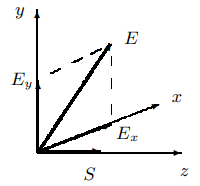
\includegraphics[width = 0.9\textwidth]{E_in_basis.png}
    \end{center}
    \caption{Представление световой волны в виде двух линейно поляризованных волн}
\end{wrapfigure}
При теоретическом рассмотрении различных типов поляризации часто бывает удобно проектировать вектор $\mathbf{E}$ в некоторой точке пространства на два взаимно перпендикулярных направления (рис. 1). В том случае, когда исходная волна была поляризованной, $E_x$ и $E_y$ когерентны между собой и могут быть записаны в виде
\begin{equation}\label{eq: E in basis}
    E_x = E_{x0}\cos(kz - \omega t), \quad
    E_y = E_{y0}\cos(kz - \omega t - \varphi),
\end{equation}
где амплитуды $E_{x0}$, $E_{y0}$, волновой вектор $k$, частота $\omega$ и сдвиг фаз $\varphi$ не зависят от времени. Немонохроматический свет может быть представлен суммой выражений типа \eqref{eq: E in basis} с различными значениями частоты $\omega$. 

Ориентация эллипса поляризации определяется отношением амплитуд $E_{y0} / E_{x0}$ и разностью фаз $\varphi$. При $\varphi = 0\text{, } \pm\pi$ эллипс вырождается в отрезок прямой. При $\varphi = \pm \pi / 2$ главные оси эллипса совпадают с осями $x$, $y$. Если при этом отношение амплитуд $E_{y0} / E_{x0} = 1$, эллипс поляризации вырождается в окружность.

В плоскости $z = z_0$ вектор $\mathbf{E}$ волны \eqref{eq: E in basis} вращается против часовой стрелки (при наблюдении навстречу волне), если $0 < \varphi < \pi$. В этом случае говорят о \textit{левой} эллиптической поляризации волны. Если же
$\pi < \varphi < 2\pi$, вращение вектора $\mathbf{E}$ происходит по часовой стрелке, и волна имеет \textit{правую} эллиптическую поляризацию

Неполяризованный свет также может быть разложен на две линейно поляризованные компоненты; однако в этом случае разность фаз $\varphi$ испытывает быстрые хаотические изменения, так что колебания $E_x$ и $E_y$ оказываются некогерентными.

\subsection{Методы получения линейно поляризованного света} 
Для получения линейно поляризованного света применяются специальные оптические приспособления -- поляризаторы. Направление колебаний электрического вектора в волне, прошедшей через поляризатор, называется \textit{разрешенным направлением} поляризатора.

Всякий поляризатор может быть использован для исследования поляризованного света. Интенсивность $I$ линейно поляризованного света после прохождения через поляризатор зависит от угла, образованного плоскостью колебаний с разрешенным направлением поляризатора:
\begin{equation}\label{eq: Malus's law}
    I = I_0\cos^2\alpha.
\end{equation}
Соотношение \eqref{eq: Malus's law} носит название закона Малюса.

Опишем несколько способов получения плоскополяризованного света.

\subsection{Отражение света от диэлектрической пластинки}
Отраженный от диэлектрика свет всегда частично поляризован. Степень поляризации света, отраженного от диэлектрической пластинки в воздух, зависит от показателя преломления диэлектрика $n$ и от угла падения $i$. Как следует из формул Френеля, полная поляризация отраженного света достигается при падении под \textit{углом Брюстера}, который определяется соотношением
\begin{equation}\label{eq: Brewster's angle}
    \tg i = n.
\end{equation}
В этом случае плоскость колебаний электрического вектора в отраженном свете перпендикулярна плоскости падения.

\subsection{Преломление света в стеклянной пластинке}
Поскольку отраженный от диэлектрической пластинки свет оказывается частично (или даже полностью) поляризованным, проходящий свет также частично поляризуется. Преимущественное направление колебаний электрического вектора в прошедшем свете совпадает с плоскостью преломления луча. Максимальная поляризация проходящего света достигается при падении под углом Брюстера. Для увеличения степени поляризации преломлённого света используют стопу стеклянных пластинок, расположенных под углом Брюстера к падающему свету.

\subsection{Преломление света в двоякопреломляющих кристаллах.}
Некоторые кристаллы обладают свойством двойного лучепреломления. Это связано
с различием поляризуемости молекул в разных направлениях.

Двоякопреломляющий кристалл называют \textit{одноосным}, если в нём существует одно направление с экстремальным значением $\varepsilon$, а в других (перпендикулярных) направлениях значения $\varepsilon$ одинаковы (тензор диэлектрической проницаемости образует эллипсоид вращения). Направления вдоль осей эллипсоида называют \textit{главными}, одно из них -- c экстремальным значением $\varepsilon$ -- \textit{оптической осью}. Линейно поляризованная волна, в которой вектор $\mathbf{E}$ перпендикулярен оптической оси, называетс я обыкновенной; если же вектор $\mathbf{E}$ имеет проекцию на оптическую ось, это необыкновенная волна. Показатели преломления этих волн обозначают через $n_o$ и $n_e$ соответственно.

Преломляясь в таких кристаллах, световой луч разделяется на два
луча со взаимно перпендикулярными плоскостями колебаний. Отклоняя один из лучей в сторону, можно получить плоскополяризованный свет, -- так устроены поляризационные призмы.

\subsection{Поглощение света в дихроических пластинках}
У некоторых двоякопреломляющих кристаллов коэффициенты поглощения света для двух взаимно перпендикулярно поляризованных лучей отличаются настолько сильно, что уже при небольшой толщине кристалла одни из лучей гасятся практически полностью, и из кристалла выходит линейно поляризованный пучок света. Это явление носит название
\textit{дихроизма}. 

Если поляроиды используются для создания поляризованного света, их называют \textit{поляризаторами}, если для определения характера поляризации -- \textit{анализаторами}.

\subsection{Определение направления разрешенной плоскости колебаний поляроида.}
При падении света на отражающую поверхность под углом Брюстера свет в отражённом луче полностью поляризован, а вектор $\mathbf{E}$ параллелен отражающей поверхности. Луч света, прошедший поляроид и отразившийс я от чёрного зеркала, имеет минимальную интенсивность при выполнении двух условий: во-первых, свет падает на отражающую поверхность под углом Брюстера, и во-вторых, в падающем пучке вектор $\mathbf{E}$ лежит в плоскости падения.

Измеряя угол Брюстера, нетрудно определить коэффициент преломления материала, из
которого изготовлено зеркало. Описанный метод часто используется для измерения
коэффициента преломления непрозрачных диэлектриков.

\subsection{Получение эллиптически поляризованного света}
Эллиптически поляризованный свет можно получить из линейно поляризованного с
помощью двоякопреломляющих кристаллических пластинок.

Двоякопреломляющая пластинка имеет два взаимно перпендикулярных \textit{главных направления}, совпадающих с осями эллипсоида диэлектрической проницаемости. Волны, поляризованные вдоль главных направлений, распространяются в пластинке с разными скоростями, не изменяя характера своей поляризации. Эти волны называются \textit{главными}. Будем обозначать показатели преломления для главных волн через
$n_\xi$ и $n_\eta$, где $\xi$ и $\eta$ -- главные направления кристаллической пластинки.

Пусть на пластинку падает линейно поляризованная волна, электрический вектор
которой ориентирован под некоторым углом $\alpha$ к оси $\xi$. Разложим вектор
$\mathbf{E}$ на составляющие $E_\xi$ и $E_\eta$. На входе пластинки $E_\xi$ и $E_\eta$ находятся в фазе. На выходе из-за разности скоростей между ними появляется разность хода, выразим её в долях длины волны
\begin{equation}\label{eq: path difference}
    \frac{\lambda}{m} = d(n_\xi - n_\eta),
\end{equation}
при этом сдвиг фаз определяется соотношением
\begin{equation}\label{eq: phase difference}
    \Delta\varphi = \frac{2 \pi}{m} = kd(n_\xi - n_\eta),
\end{equation}
где $k$ -- волновое число для вакуума, $d$ -- толщина кристаллической пластинки.
\begin{wrapfigure}[19]{r}{0.4\textwidth}\label{fig: E in crystall}
    \begin{center}
    \vspace{-20pt}
        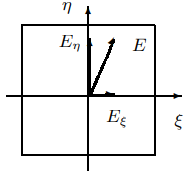
\includegraphics[width = 0.9\textwidth]{E_in_crystall.png}
    \end{center}
    \caption{Разложение линейно поляризованного света по главным направлениям двоякопреломляющей пластинки}
\end{wrapfigure}

Рассмотрим практически важные частные случаи.

a) Пластинка дает сдвиг фаз $2\pi$ (пластинка в длину волны). В результате сложения волн на выходе пластинки образуется линейно поляризованная волна с тем же направлением колебаний, что и в падающей волне.

б) Пластинка дает сдвиг фаз $\pi$ (пластинка в полдлины волны). На выходе пластинки снова образуется линейно поляризованная волна. Направление колебаний этой волны является отражением направления колебаний падающей волны относительно одного из главных направлений пластинки.

в) Пластинка создает между колебаниями сдвиг фаз $\pi / 2$ (пластинка в четверть длины волны). При сложении двух взаимно перпендикулярных колебаний, имеющих разность фаз $\pi / 2$, образуется эллипс, главные оси которого совпадают с координатными осями $\xi$ и $\eta$. При равенстве амплитуд $E_{\xi 0}$ = $E_{\eta 0}$ возникает круговая поляризация.

Следует отметить, что, говоря о пластинках $\lambda$, $\lambda / 2$, $\lambda / 4$ ..., всегда подразумевают какую-либо вполне определенную монохроматическую компоненту. Если на двоякопреломляющую пластинку падает не монохроматический свет, то на выходе из нее для разных спектральных компонент эллипсы поляризации будут различными.

\subsection{Анализ эллиптически поляризованного света}
Анализ эллиптически поляризованного света сводится к нахождению главных осей эллипса поляризации и к определению направления вращения электрического вектора.

Главные оси эллипса поляризации определяются с помощью анализатора по максимуму и минимуму интенсивности проходящего света. Направление вращения электрического вектора может быть найдено с помощью пластинки в четверть длины волны, для которой известно, какая из главных волн, $E_\xi$ или $E_\eta$, имеет большую скорость распространения.

Поместим такую пластинку на пути эллиптически поляризованного света и совместим главные оси эллипса поляризации с главными направлениями пластинки $\lambda / 4$. На выходе из этой
пластинки сдвиг фаз между $E_\xi$ и $E_\eta$ вместо $\pi / 2$ станет равным нулю или $\pi$, свет окажется линейно поляризованным. Если фаза на выходе станет нулевой, то значит пластинки cкомпенсировали друг друга и направления вращения на эллипсах в них разные. Иначе, направления совпадают.

\subsection{Интерференция поляризованных лучей}
Тонкие двоякопреломляющие пластинки, помещенные между поляроидами, кажутся окрашенными. Эта окраска может быть истолкована как результат интерференции поляризованных лучей. 

Если поворачивать двоякопреломляющую пластинку, расположенную между скрещенными поляроидами, то соотношение амплитуд волн и разность фаз между ними не изменяются. Это означает, что цвет пластинки при ее поворотах не меняется, а меняется только интенсивность света. За один оборот пластинки интенсивность четыре раза обращается в нуль, -- это происходит при совпадении главных направлений $\xi$ и $\eta$ с разрешенными направлениями колебаний поляроидов.

Если же двоякопреломляющую пластинку оставить неподвижной, а второй поляроид вращать, то волны и приобретают дополнительный фазовый сдвиг для всех спектральных компонент; поэтому цвет пластинки изменится на дополнительный.

%\section{Экспериментальная установка}

\section{Обработка данных}  
\begin{enumerate}
    \item 
    Сначала определим разрешённые направления поляроидов. Для этого разместим на оптической скамье осветитель $S$, поляроид $P_1$ и чёрное зеркало так, чтобы плоскость падения была горизонтальна, после этого свет, отражённый от зеркала, будем рассматривать сбоку. Поворачивая поляроид вокруг направления луча, добьёмся наименьшей яркости отражённого пятна, после этого вращением зеркала вокруг вертикальной оси снова добьёмся минимальной интенсивности отражённого луча. Запишем значение угла для поляроида $P_1$.
    \begin{figure}[H]\label{fig: Polaroid_directions}
        \centering
        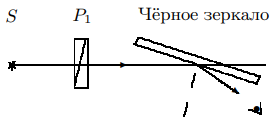
\includegraphics[width = 0.6\textwidth]{Polaroid_directions.png}
        \caption{Определение разрешённого направления поляроида}
    \end{figure}

    Разрешённое направление второго поляроида определим, скрестив поляроиды: после поляроида с известной поляризацией поставим второй поляроид и, глядя навстречу лучу, вращением второго поляроида получим минимальную яркость луча. Запишем значение для полученного направления $P_2$. Результаты отсчёта по лимбу приведены в таблице ниже.
    \begin{table}[H]\label{tab: Polarization angles}
        \centering
        \begin{tabular}{|
            >{\columncolor[HTML]{FFFFFF}}c |
            >{\columncolor[HTML]{FFFFFF}}c |
            >{\columncolor[HTML]{FFFFFF}}c |}
            \hline
            {\color[HTML]{000000} Поляроид}    & {\color[HTML]{000000} $P_1$}               & {\color[HTML]{000000} $P_2$}                 \\ \hline
            {\color[HTML]{000000} Отсчёт}      & {\color[HTML]{000000} $30\degree$}         & {\color[HTML]{000000} $83\degree$}           \\ \hline
            {\color[HTML]{000000} Поляризация} & {\color[HTML]{000000} В плоскости падения} & {\color[HTML]{000000} Перпендикулярно плоскости падения} \\ \hline
        \end{tabular}
        \caption{Значения углов и поляризаций для $P_1$ и $P_2$}
    \end{table}

    \item
    Далее с помощью угла Брюстера определим показатель преломления эбонита. Для этого, с помощью поляризатора $P_1$, оставим только свет, поляризованный в плоскости падения и найдём угол поворота эбонита $\varphi_б$, при котором интенсивность отражённого луча минимальна, добавив зелёный фильтр, повторим измерения. По углу Брюстера, используя формулу \eqref{eq: Brewster's angle}, рассчитаем показатель преломления эбонита.
    \begin{table}[H]\label{tab: Brewsters angle}
        \centering
        \begin{tabular}{|
            >{\columncolor[HTML]{FFFFFF}}c |
            >{\columncolor[HTML]{FFFFFF}}c |
            >{\columncolor[HTML]{FFFFFF}}c |}
            \hline
            {\color[HTML]{000000} }              & {\color[HTML]{000000} Без фильтра} & {\color[HTML]{000000} С фильтром}  \\ \hline
            {\color[HTML]{000000} Угол Брюстера} & {\color[HTML]{000000} $57\degree$} & {\color[HTML]{000000} $55\degree$} \\ \hline
        \end{tabular}
        \caption{Угол Брюстера для эбонита}
    \end{table}
    \[n = \tg\varphi_б \approx 1,54\]
    Табличное значение показателя преломления: $n = 1.6$.
    \begin{figure}[H]\label{fig: Black_mirror}
        \centering
        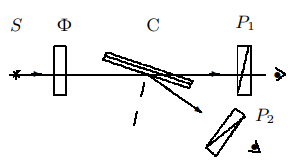
\includegraphics[width = 0.6\textwidth]{Black_mirror.png}
        \caption{Исследование стопы}
    \end{figure}
    
    \item 
    Теперь исследуем стопу стеклянных пластинок. Поставим стопу вместо эбонитового зеркала и  
    подберём для неё угол Брюстера. После этого, с помощью поляризаторов $P_1$ и $P_2$, определим характер поляризации света в отражённом и преломлённом лучах. Видим, что так как свет падает на пластинки под углом Брюстера, то в отражённом свете получаем поляризацию, при которой вектор $\mathbf{E}$ лежит вне плоскости падения. В преломлённом свете, из-за большого количества стеклянных пластинок, получаем приемущественно поляризацию, где вектор $\mathbf{E}$ лежит в плоскости падения.

    \item
    В этом пункте определим главные плоскости двоякопреломляющих пластин. Для этого между скрещенными поляроидами расположим кристаллическую пластинку. Вращая пластинку вокруг направления луча и наблюдая за интенсивностью света, проходящего сквозь второй поляроид, определим, когда наблюдается минимум интенсивности. В таком случае направления пластинки совпадают с разрешёнными направлениями поляроидов. Сведём результаты в таблицу.
    \begin{table}[H]\label{tab: main axises}
        \centering
        \begin{tabular}{|
            >{\columncolor[HTML]{FFFFFF}}c |
            >{\columncolor[HTML]{FFFFFF}}c |
            >{\columncolor[HTML]{FFFFFF}}c |}
            \hline
            {\color[HTML]{000000} }                  & {\color[HTML]{000000} Пластинка 1}  & {\color[HTML]{000000} Пластинка 2}                         \\ \hline
            {\color[HTML]{000000} Положение главных осей} & {\color[HTML]{000000} $180\degree$} & \cellcolor[HTML]{FFFFFF}{\color[HTML]{000000} $97\degree$} \\ \hline
        \end{tabular}
        \caption{Значения углов главных осей пластинок}
    \end{table}
    \begin{figure}[H]\label{fig: Main_directions}
        \centering
        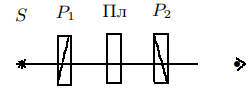
\includegraphics[width = 0.6\textwidth]{Main_directions.png}
        \caption{Определение главных направлений в пластинках}
    \end{figure}

    \item
    Далее определим какая из пластин соответствует разности фаз $\pi$, а какая разности фаз $\pi / 2$. Для этого добавим к схеме зелёный фильтр, установим разрешённое направление поляроида горизонтально, а главные направления исследуемой пластинки -- под углом $45\degree$ к горизонтали. С помощью второго поляроида установим, какую поляризацию имеет свет, прошедший пластинку. Если пластинка $\lambda / 4$, то поляризация будет круговой и при любом положении второго поляризатора интенсивность будет одинаковой. Если пластинка $\lambda / 2$, то поляризация будет линейной будет существовать положение второго поляризатора при котором интенсивность будет обращаться в ноль. Результаты приведены в таблице ниже.
    \begin{table}[H]\label{tab: lmbds for plates}
        \centering
        \begin{tabular}{|
            >{\columncolor[HTML]{FFFFFF}}c |
            >{\columncolor[HTML]{FFFFFF}}c |
            >{\columncolor[HTML]{FFFFFF}}c |}
            \hline
            {\color[HTML]{000000} }           & {\color[HTML]{000000} Пластинка 1}   & {\color[HTML]{000000} Пластинка 2}   \\ \hline
            {\color[HTML]{000000} Сдвиг фазы} & {\color[HTML]{000000} $\lambda / 4$} & {\color[HTML]{000000} $\lambda / 2$} \\ \hline
        \end{tabular}
        \caption{Сдвиг фаз для каждой из пластинок}
    \end{table}

    \item
    Наконец, найдём направлений большей и меньшей скорости в пластинке $\lambda / 4$. Для этого поставим между скрещенными поляроидами пластинку чувствительного оттенка ($\lambda$ для зелёного света). Установим разрешённое направление первого поляроида горизонтально. Добавим к схеме пластинку $\lambda / 4$, главные направления которой совпадают с главными направлениями пластины $\lambda$ и ориентированы под углом $45\degree$ к разрешённым направлениям скрещенных поляроидов. При повороте рейтера на $180\degree$ вокруг вертикальной оси цвет стрелки меняется от оранжево-жёлтого до сине-зелёного, в первом случае «быстрые» оси стрелки и пластинки не совпадают, во втором совпадают.  
    \begin{figure}[H]\label{fig: Speed_directions}
        \centering
        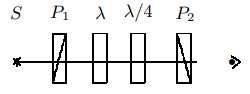
\includegraphics[width = 0.6\textwidth]{Speed_directions.png}
        \caption{Определение направлений большей и меньшей скорости}
    \end{figure}

    \item
    Теперь определим направления вращения светового вектора в эллиптически поляризованной волне. Поставим зелёный фильтр, а за ним между скрещенными поляроидами -- пластинку  толщины $\lambda / 4$. Получим эллиптически поляризованный свет. Для этого установим разрешённое направление первого поляроида под углом $10\degree-20\degree$ к горизонтали так, чтобы вектор $\mathbf{E}$ падающего на пластинку света был расположен в первом квадранте. Разрешённое направление второго поляроида установим вертикально, и, вращая пластинку, найдём минимум интенсивности света, прошедшего через второй поляроид. Таким образом мы получили эллиптически поляризованный свет с вертикальной малой осью. 

    Для определения направления вращения светового вектора в эллипсе установим между поляроидами дополнительную пластинку $\lambda / 4$ с известными направлениями «быстрой» и «медленной» осей, ориентированными по осям эллипса поляризации анализируемого света. В этом случае вектор $\mathbf{E}$ на выходе будет таким, как если бы свет прошел две пластинки $\lambda / 4$: свет на выходе из второй пластинки будет линейно поляризован. Если пластинки поодиночке дают эллипсы, вращающиеся в разные стороны, то поставленные друг за другом, они скомпенсируют разность фаз, и вектор $\mathbf{E}$ на выходе останется в первом и третьем квадрантах. Если же световой вектор перешёл в смежные квадранты, значит, эллипсы вращаются в одну сторону.

    После второго поляроида интенсивность света максимальна в первом квадранте. Значит, две пластины компенсируют друг друга и эллипсы вращаются в разные сторону.

    \begin{figure}[H]\label{fig: Sinuses}
        \centering
        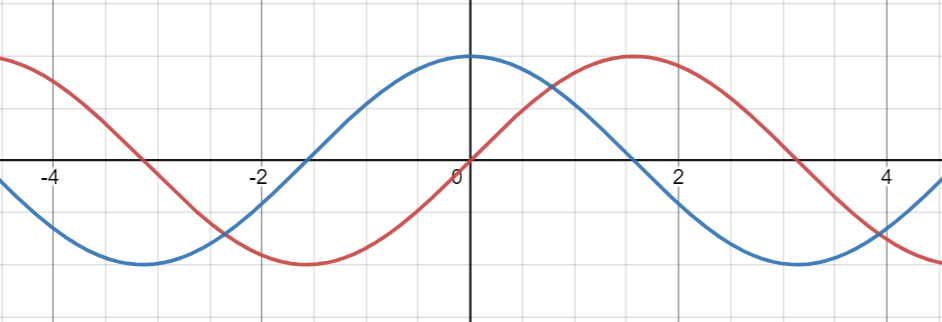
\includegraphics[width = 0.8\textwidth]{Sinuses.png}
        \caption{Синусы с разностью фаз $\pi / 2$}
    \end{figure}

    \item
    В последнем пункте расположим между скрещенными поляроидами мозаичную слюдяную пластинку. Она собрана из 4-х узких полосок слюды, лежащих по сторонам квадрата (две полоски «толщиной» $\lambda / 4$ и по одной -- $\lambda / 2$ и $3 \lambda / 4$). Главные направления всех пластинок ориентированы параллельно сторонам квадрата.

    Сначала будем вращать пластинку и наблюдать за изменениями в отдельном квадратике. Видим, что при этом меняется интенсивность в каждом квадрате, но цвет остаётся неизменным.

    Теперь, не трогая пластинки, будем вращать второй поляроид. При этом в каждом квадратике меняется интенсивность света, а также при переходе через определённое значение угла поворота второго поляроида меняется цвет.
 
\end{enumerate}

\newpage
\section{Вывод}
В данной работе были получены следующие результаты:
\begin{itemize}
    \item 
    Определены разрешённые направления каждого из поляроидов -- для первого поляроида $P_1$ отсчёт по лимбу -- $30\degree$, для второго $P_2$ -- $83\degree$.
    
    \item 
    По углу Брюстера был определён показатель преломления эбонита, полученное значение хорошо совпадает с табличным:
    \[n = \tg\varphi_б \approx 1,54, \quad n_{табл} = 1,6.\]
    
    \item
    С помощью стопы стеклянных пластинок были получены различные поляризации в отраженном и преломленном свете.

    \item
    Были определены главные направления двоякопреломляющих пластин, для первой пластинки значение угла, при котором оси совпадают с горизонталью и вертикалью, -- $180\degree$, для второй -- $97\degree$.

    \item
    С помощью второго поляризатора было выяснено, что первая из пластин есть пластинка $\lambda / 4$, вторая -- $\lambda / 2$.

    \item
    Было определено, какая из главных осей пластинки является «быстрой» осью, а какая есть «медленная».  

    \item
    Было определено направление вращения вектора $\mathbf{E}$ в эллиптически поляризованном свете: пластинка $\lambda / 4$ компенсирует разность фаз со второй пластинкой, следовательно эллипсы этих пластинок вращаются в разные стороны.
    
    \item
    При изучении интерференции поляризованных лучей было получено, что при вращении пластинки меняется только интенсивность света в каждом квадратике. Если же вращать второй поляроид, не трогая пластинку, меняется как интенсивность, так и цвет.
    
\end{itemize}

%%%%%%%%%%%%%%%%%%%%%%%%% Графики
\newpage

%%%%%%%%%%%%%%%%%%%%%%%%%
\end{document}
